\documentclass[conference,letterpaper]{IEEEtran}

\usepackage{amsmath,amssymb,amsfonts}
\usepackage{graphicx}
\usepackage{booktabs}
\usepackage{tabularx}
\usepackage{algorithm}
\usepackage{algpseudocode}
\usepackage{url}
\usepackage{cite}
\usepackage{microtype}
\usepackage{enumitem}
\setlist{nosep, leftmargin=*}

% Caption styling for IEEE compliance
\makeatletter
\def\fnum@figure{Fig.~\thefigure}
\makeatother

% Compact float spacing to balance column height
\setlength{\textfloatsep}{5pt plus 1pt minus 1pt}
\setlength{\dbltextfloatsep}{5pt plus 1pt minus 1pt}
\setlength{\floatsep}{4pt plus 1pt minus 1pt}
\setlength{\intextsep}{4pt plus 1pt minus 1pt}

% Compact bibliography item separation
\let\oldthebibliography\thebibliography
\let\endoldthebibliography\endthebibliography
\renewenvironment{thebibliography}[1]{%
  \begin{oldthebibliography}{#1}%
    \setlength{\itemsep}{0.5pt}%
    \setlength{\parskip}{0pt}%
}{%
  \end{oldthebibliography}%
}

\begin{document}

\title{\textbf{An Intelligent Agent for Phishing Simulation and Behavioral Threat Analysis}}

\author{
  \IEEEauthorblockN{Manitej, Ch. Avinash, K. Mani Tej Kumar, K. Kowshik}
  \IEEEauthorblockA{Department of Cyber Security\\
  Malla Reddy University, Hyderabad, Telangana, India}
}

\maketitle

\begin{abstract}
\textbf{Abstract}---Phishing attacks remain among the most prevalent cyber threats, primarily because they exploit human trust, cognitive biases, and organizational pressure rather than technical vulnerabilities. Conventional security awareness programs typically rely on generic, infrequent training sessions that measure administrative completion rates instead of observable behavioral responses. In this work, we present SemanticShield AI, an intelligent agent framework designed for phishing simulation and behavioral threat analysis. The system allows security trainers to configure specific attack scenarios, target organizational roles, and distinct behavioral personas---including Trusting HR Managers, Security-Conscious Developers, Overwhelmed Finance Managers, and Executives. For each simulation, an intelligent persona evaluates the email payload using the Gemini API, producing transparent reasoning followed by an explicit safety decision. These decisions map directly to threat scores that are integrated into a centralized risk engine, classifying incidents as Safe, Suspicious, or Dangerous while maintaining complete isolation between simulation data and operational detections. Across 63 empirical evaluation runs against a credential-harvesting scenario, behavioral profiles exhibited distinct vulnerability distributions, ranging from 100\% susceptibility in trusting personas to 50\% in security-conscious profiles. The entire platform operates in a synthetic environment without transmitting emails to real employees, providing actionable defensive insights while strictly upholding organizational ethics.
\end{abstract}

\begin{IEEEkeywords}
\textit{Index Terms}---Phishing simulation, behavioral threat analysis, intelligent agents, large language models, social engineering, security awareness training, automated vulnerability assessment, persona modeling.
\end{IEEEkeywords}

\section{INTRODUCTION}
Enterprise communication channels face relentless offensive probing, with social engineering persisting as the predominant entry point for corporate network infiltration. Although perimeter defenses such as spam filters and security gateways intercept malicious emails in bulk, sophisticated threat actors craft targeted messages that bypass heuristic and statistical filters. These attacks intentionally target human psychological vulnerabilities, exploiting organizational hierarchy, procedural familiarity, personal benevolence, and cognitive fatigue under urgent workplace deadlines.

Automated computational entities capable of perceiving operational environments and formulating rational defensive responses are rooted in foundational artificial intelligence research. As formalized by Russell and Norvig \cite{russell2021}, intelligent agents operate by observing environmental states through percepts and executing actions that maximize expected performance measures. The theoretical grounding of autonomous agency, cooperative multi-agent dynamics, and goal-directed behavioral reasoning was established by Wooldridge and Jennings \cite{wooldridge1995}, providing the conceptual architecture for autonomous decision systems interacting with structured and unstructured stimuli.

Recent transformations in natural language processing have established generative foundation models capable of complex contextual comprehension. In their seminal work, Brown et al. \cite{brown2020} demonstrated that large language models exhibit robust few-shot learning capabilities, adapting to specialized reasoning domains without parameter updates when supplied with structured instructional conditioning. These capabilities were extended through contextual groundings and external information retrieval formulations investigated by Lewis et al. \cite{lewis2020}. A comprehensive survey of modern architectural advances, reasoning paradigms, and behavioral alignment mechanisms across language models was compiled by Zhao et al. \cite{zhao2023}, documenting the emergence of nuanced persona emulation and human-like deduction under diverse prompt constraints.

Despite advances in artificial intelligence, organizational defenses remain severely compromised by the human element. The seminal investigation by Dhamija, Tygar, and Hearst \cite{dhamija2006} proved that phishing succeeds primarily because visual deception exploits cognitive heuristics, demonstrating that even educated computer users routinely fail to identify spoofed domains and fraudulent visual authenticators. Early attempts to mitigate these cognitive blind spots through embedded training methodologies were explored by Kumaraguru et al. \cite{kumaraguru2010}, who demonstrated that instructional materials delivered immediately following user interaction significantly outperform passive classroom instruction. Gamified instructional designs were subsequently developed by Sheng et al. \cite{sheng2007}, demonstrating measurable reductions in click-through rates when training engages active procedural memory.

Nevertheless, human vulnerability to deception remains a persistent organizational reality. In his systematic analysis of interpersonal deception, Hadnagy \cite{hadnagy2018} documented how social engineers weaponize fundamental psychological principles---including cognitive authority, social proof, reciprocity, and induced urgency---to compel employees into violating security protocols. The strategic significance of these human attack vectors is underscored by empirical telemetry from industry breach studies. The 2024 Data Breach Investigations Report published by Verizon \cite{verizon2024} established that the human element continues to be involved in an overwhelming majority of commercial data breaches, with phishing and pretexting ranking among the top three initial access methods across all recorded enterprise security compromises.

Conventional Security Awareness Training (SAT) platforms suffer from severe structural deficiencies. Most corporate environments administer compliance training on a rigid annual schedule, relying on passive video lectures and multiple-choice questionnaires. These instruments measure administrative course completion rather than authentic behavioral resilience. When organizations attempt live phishing simulations by dispatching spoofed emails to actual employees, the exercises frequently introduce workplace friction, erode trust between staff and internal security teams, and produce binary click-rate metrics that offer no visibility into the cognitive rationale behind an employee's failure.

To address these systemic shortcomings, this paper presents SemanticShield AI, an intelligent agent platform for synthetic phishing simulation and behavioral threat analysis. SemanticShield AI introduces a simulation methodology where security trainers execute simulated phishing attacks against autonomous AI personas that emulate realistic workplace roles and cognitive profiles. The agentic reasoning pipeline is powered by the Gemini API \cite{gemini2024}, which receives detailed cognitive persona prompts alongside the candidate email payload, generates step-by-step reasoning, and yields a standardized safety decision. The operational backend is constructed using FastAPI \cite{fastapi2024} to deliver asynchronous request processing and streaming telemetry, while relational data integrity and schema management are guaranteed by SQLAlchemy and Alembic \cite{sqlalchemy2024}.

The primary technical contributions of this research are:
\begin{enumerate}
    \item We design an autonomous agent framework leveraging the Gemini API \cite{gemini2024} to emulate diverse employee behavioral archetypes (Trusting HR Manager, Security-Conscious Developer, Overwhelmed Finance Manager, and Executive Vice President).
    \item We develop a transparent chain-of-thought simulation protocol that outputs granular cognitive reasoning followed by strict decision markers (\texttt{[VULNERABLE]} or \texttt{[SAFE]}), enabling security personnel to inspect the exact cognitive steps leading to a compromise.
    \item We formulate a calibrated threat scoring integration that maps binary agent outcomes into numerical threat metrics ($85$ for vulnerable, $15$ for safe), directly feeding an organizational risk engine to categorize threat severities into Safe, Suspicious, or Dangerous tiers.
    \item We ensure complete ethical isolation: simulations are conducted entirely in a synthetic runtime without sending emails to real users, persisting records with strict operational separation (\texttt{is\_simulation = true}).
    \item We conduct an empirical evaluation consisting of 63 experimental runs across the four behavioral personas against an identical Microsoft 365 credential-harvesting payload, analyzing susceptibility distributions, severity outputs, confidence metrics, and processing latencies.
\end{enumerate}

The remainder of this paper is structured as follows. Section II reviews related literature. Section III defines the problem, design objectives, existing approaches, and the proposed system model. Section IV presents the system architecture, simulation data flow, and formal execution algorithm. Section V details the methodology, persona definitions, reasoning extraction, threat scoring, and system requirements. Section VI presents experimental findings, comparative charts, qualitative demonstration runs, and research limitations. Section VII concludes the paper and identifies future extensions.

\section{LITERATURE SURVEY}

\subsection{Phishing and Human Factors}
The resilience of computer systems is fundamentally constrained by human decision-making processes. In their empirical study, Dhamija, Tygar, and Hearst \cite{dhamija2006} investigated why phishing strategies remain effective against diverse user demographics. Their findings revealed that visual deception successfully exploits psychological tendencies, such as surface credibility and brand trust, while users frequently ignore or misinterpret security indicators like digital certificates and domain structures. Users tend to rely on cognitive heuristics, equating visual professional presentation with authentic corporate legitimacy. These psychological vulnerabilities are systematically exploited in social engineering operations. Hadnagy \cite{hadnagy2018} categorized the primary persuasion vectors utilized by social engineers, demonstrating that cognitive load, workplace stress, and perceived authority diminish an individual's analytical verification capacity. When an email invokes severe urgency---such as an impending account suspension or a wire transfer deadline---the recipient's cognitive processing shifts from reflective analytical reasoning to automatic, heuristic-driven compliance. Furthermore, as documented in the Verizon 2024 Data Breach Investigations Report \cite{verizon2024}, credential harvesting and social engineering represent primary drivers of enterprise breach incidents, demonstrating that perimeter defenses are routinely bypassed when authorized user credentials are voluntarily surrendered.

\subsection{Security Awareness Training}
To counteract the threat of social engineering, enterprise organizations routinely deploy Security Awareness Training (SAT) programs. Early foundational studies by Kumaraguru et al. \cite{kumaraguru2010} explored active learning methodologies, comparing standard passive instructional materials against embedded training systems. Their research, centered on the ``PhishGuru'' framework, demonstrated that training interventions delivered immediately following an employee's interaction with a simulated phishing message produce significantly higher retention rates and behavioral adaptation than traditional classroom training. Building upon cognitive instructional theory, Sheng et al. \cite{sheng2007} developed and evaluated ``Anti-Phishing Phil,'' an interactive game designed to teach users how to inspect Uniform Resource Locators (URLs) and identify spoofed hostnames. Their experiments demonstrated that interactive, scenario-based learning mechanisms cultivate superior threat identification skills compared to reading static web pages or compliance handbooks. However, existing enterprise implementations of SAT suffer from pronounced operational flaws. Current commercial programs are predominantly compliance-centric, measuring program success via completion percentages of annual slide decks. When organizations deploy live phishing tests targeting actual employees, they often inadvertently generate friction, employee resentment, and reduced organizational productivity.

\subsection{Intelligent Agents and Language Models}
The formalization of intelligent agents as computational systems capable of flexible autonomous action within dynamic environments was articulated by Russell and Norvig \cite{russell2021}. An intelligent agent continuously perceives its environment, updates internal state representations, and selects actions governed by an optimization function or goal state. Wooldridge and Jennings \cite{wooldridge1995} defined the essential properties of agenthood as autonomy, social ability, reactivity, and pro-activeness, providing the conceptual foundation for simulating human behavioral characteristics in synthetic computational environments. The evolution of generative artificial intelligence has unlocked unprecedented capabilities for modeling human linguistic and cognitive behavior. Brown et al. \cite{brown2020} demonstrated that large language models trained on massive text corpora exhibit emergent reasoning capabilities, enabling few-shot and zero-shot task completion guided entirely by natural language instructions. The integration of contextual reasoning frameworks was further advanced by Lewis et al. \cite{lewis2020}, who demonstrated that conditioning model outputs on structured external contexts enhances factual accuracy and domain specificity. In their comprehensive survey, Zhao et al. \cite{zhao2023} categorized large language model architectures, emergent abilities, and prompt engineering strategies, highlighting the capacity of advanced foundation models to execute complex chain-of-thought deductions without human intervention.

\subsection{Software Foundations}
Implementing an agentic simulation system capable of real-time behavioral modeling requires a high-performance, asynchronous software infrastructure. The generative inference pipeline relies on modern generative interfaces provided by the Gemini API \cite{gemini2024}, which supports high-throughput token streaming, structured persona parameter conditioning, and deterministic temperature controls. At the application layer, asynchronous communication and rigorous data validation are essential for handling concurrent simulation workflows. Ram\'irez \cite{fastapi2024} established architectural patterns for high-performance Python web services using FastAPI. FastAPI leverages Python type hints and Pydantic validation schemas to guarantee strict input sanitation at runtime, while native asynchronous event loops provide low-latency request dispatching and WebSocket streaming. For the persistence tier, relational integrity, transactional isolation, and schema version control are critical. The SQLAlchemy and Alembic projects \cite{sqlalchemy2024} provide declarative Object-Relational Mapping (ORM) and automated schema migration management. These tools ensure that experimental simulations, risk calculations, and audit logs are safely stored in structured database environments with transactional isolation.

\section{PROBLEM DEFINITION AND DESIGN OBJECTIVES}

\subsection{Problem Definition}
Phishing attacks succeed primarily by manipulating human trust, authority deference, and cognitive fatigue rather than breaking cryptographic primitives. Traditional organizational countermeasures rely on annual compliance modules that assess course completion checkboxes rather than practical behavioral habits. When organizations deploy live phishing tests against their own workforces, they introduce operational friction, foster employee distrust toward IT security teams, and record binary click rates without revealing the cognitive reasoning behind user failures. There is an urgent need for an automated, explainable, and ethically sound simulation framework that evaluates attack payloads against diverse cognitive profiles in an isolated sandbox.

\subsection{Design Objectives}
To address these limitations, SemanticShield AI was designed around five primary engineering objectives:
\begin{enumerate}
    \item \textbf{Cognitive Persona Simulation:} Emulate realistic employee behaviors across diverse organizational roles, capturing distinct cognitive habits, verification routines, and failure modes.
    \item \textbf{Explainable Step-by-Step Reasoning:} Generate granular, transparent chain-of-thought analysis for every simulation run, revealing the exact cognitive steps that lead to safe or vulnerable outcomes.
    \item \textbf{Calibrated Threat and Risk Integration:} Translate binary persona decisions into standardized threat scores that integrate into enterprise risk scoring engines using clear severity tiers (Safe, Suspicious, Dangerous).
    \item \textbf{Strict Operational and Ethical Containment:} Execute all evaluations entirely in a synthetic sandbox without transmitting emails to real users, ensuring that simulation records remain strictly isolated from live operational incidents (\texttt{is\_simulation = true}).
    \item \textbf{Real-Time Streaming Telemetry:} Deliver live simulation reasoning and decision markers over WebSocket connections to an interactive trainer interface, providing instant feedback.
\end{enumerate}

\begin{table}[t]
\caption{Comparison of Existing Security Approaches and Proposed Behavioral Simulation}
\label{tab:comparison}
\centering
\renewcommand{\arraystretch}{0.90}
\begin{tabularx}{\columnwidth}{lXp{1.9cm}}
\toprule
\textbf{Approach} & \textbf{Operational Mechanism} & \textbf{Key Limitation / Gap} \\
\midrule
Manual Spreadsheets & Static roster tracking; manual record keeping & No behavioral insight; static, labor-intensive, quickly obsolete \\
\addlinespace
Fixed-Template Platforms & Automated mass mailings using static templates & High employee friction; binary click metric; zero cognitive reasoning \\
\addlinespace
Generic Awareness Courses & Annual compliance videos and multiple-choice quizzes & Measures administrative compliance, not real behavioral habit \\
\addlinespace
\textbf{Proposed System} & \textbf{Synthetic LLM personas evaluating attack emails} & \textbf{Explainable reasoning; zero employee friction; continuous risk assessment} \\
\bottomrule
\end{tabularx}
\end{table}

\subsection{Existing Approaches and Their Limitations}
Table \ref{tab:comparison} summarizes the primary existing organizational approaches and identifies the critical gaps addressed by this research. Manual spreadsheets rely on static rosters, tracking training dates without assessing real employee capability. Fixed-template simulation platforms dispatch pre-authored phishing emails across corporate mailboxes; while they measure click rates, they provoke employee frustration and offer no explanatory insight into the cognitive mechanisms behind a user's failure. Generic awareness courses rely on passive multiple-choice evaluations that verify superficial compliance rather than behavioral security habits. In contrast, the proposed SemanticShield AI platform deploys intelligent AI personas to evaluate attack emails in a synthetic sandbox, generating granular reasoning and calibrated threat metrics with zero disruption to employees.

\subsection{Proposed System}
SemanticShield AI establishes an automated simulation pipeline that replaces live employee deception with synthetic, persona-driven evaluation. The security trainer interacts with a single-page React interface, configuring the simulation by selecting a phishing attack scenario, an employee organizational role, a behavioral profile, and the email payload (subject and body). Upon submission, the request is validated by a FastAPI backend and transmitted to the Gemini API \cite{gemini2024} with a specialized system prompt that conditions the model to adopt the selected behavioral persona. The model streams its reasoning in real time over WebSockets and emits an explicit decision marker (\texttt{[VULNERABLE]} or \texttt{[SAFE]}). The decision maps to a quantitative threat score, passes through a risk engine, and is persisted in an SQLite database via SQLAlchemy with the flag \texttt{is\_simulation = true}.

\section{SYSTEM ARCHITECTURE AND DESIGN}

\subsection{Overall Architecture}
The architectural structure of SemanticShield AI is organized as a three-tier modular system, depicted in Fig. 1. The architecture cleanly separates user interaction, application intelligence, risk calculation, and transactional persistence.

\begin{figure}[t]
\centering
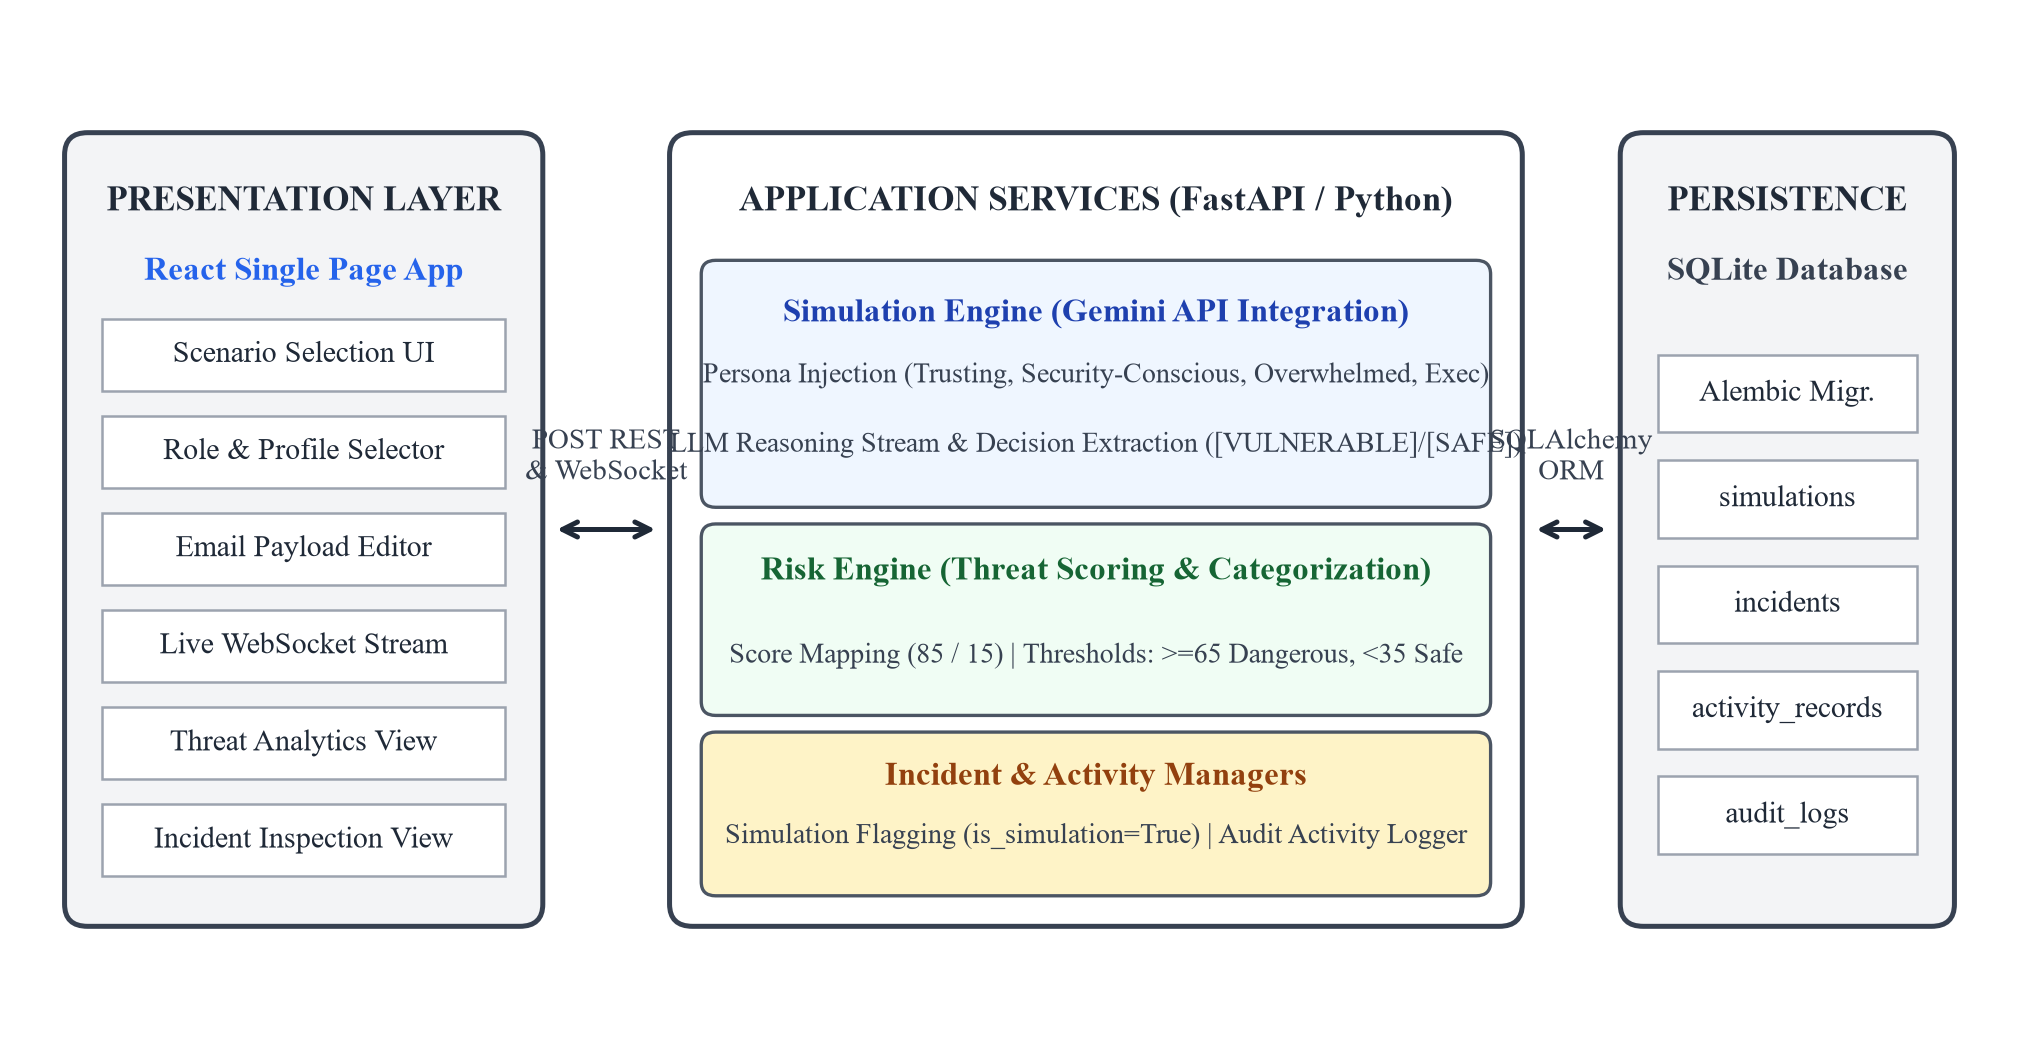
\includegraphics[width=0.82\columnwidth, height=2.6cm, keepaspectratio]{figures/fig1.png}
\caption{Architecture of SemanticShield AI showing the simulation engine, the risk engine, the incident and activity managers, the persistence layer, and the frontend.}
\label{fig:architecture}
\end{figure}

The \textbf{Presentation Layer} consists of an interactive React single-page application. It provides input controls for scenario selection, role and profile configuration, and email payload authoring. It also renders the live reasoning stream over a persistent WebSocket connection, accompanied by risk severity gauges and analytics dashboards.

The \textbf{Application Layer} is built with FastAPI \cite{fastapi2024} running on Python 3.10 or later. It contains four core sub-modules:
\begin{enumerate}
    \item \textit{Phishing Simulation Engine:} Orchestrates the simulation lifecycle, constructs the persona prompt, communicates with the Gemini API \cite{gemini2024}, and parses the final decision.
    \item \textit{Risk Engine:} Evaluates the extracted simulation outcome, maps the decision to a numerical threat score, and applies severity threshold rules.
    \item \textit{Incident Manager:} Instantiates an isolated incident record, ensuring that simulated events are flagged with \texttt{is\_simulation = true}.
    \item \textit{Activity Manager:} Emits real-time event logs into the audit feed, tracking trainer actions and simulation completions.
\end{enumerate}

The \textbf{Persistence Layer} utilizes an SQLite relational database managed through SQLAlchemy ORM and Alembic migration tracking \cite{sqlalchemy2024}. The database maintains distinct tables for simulation records, security incidents, activity feeds, and configuration metadata.

\subsection{Simulation Data Flow}
The sequence of data transformations occurring during an active simulation run is illustrated in Fig. 2. The flow progresses linearly through five distinct phases:

\begin{figure}[t]
\centering
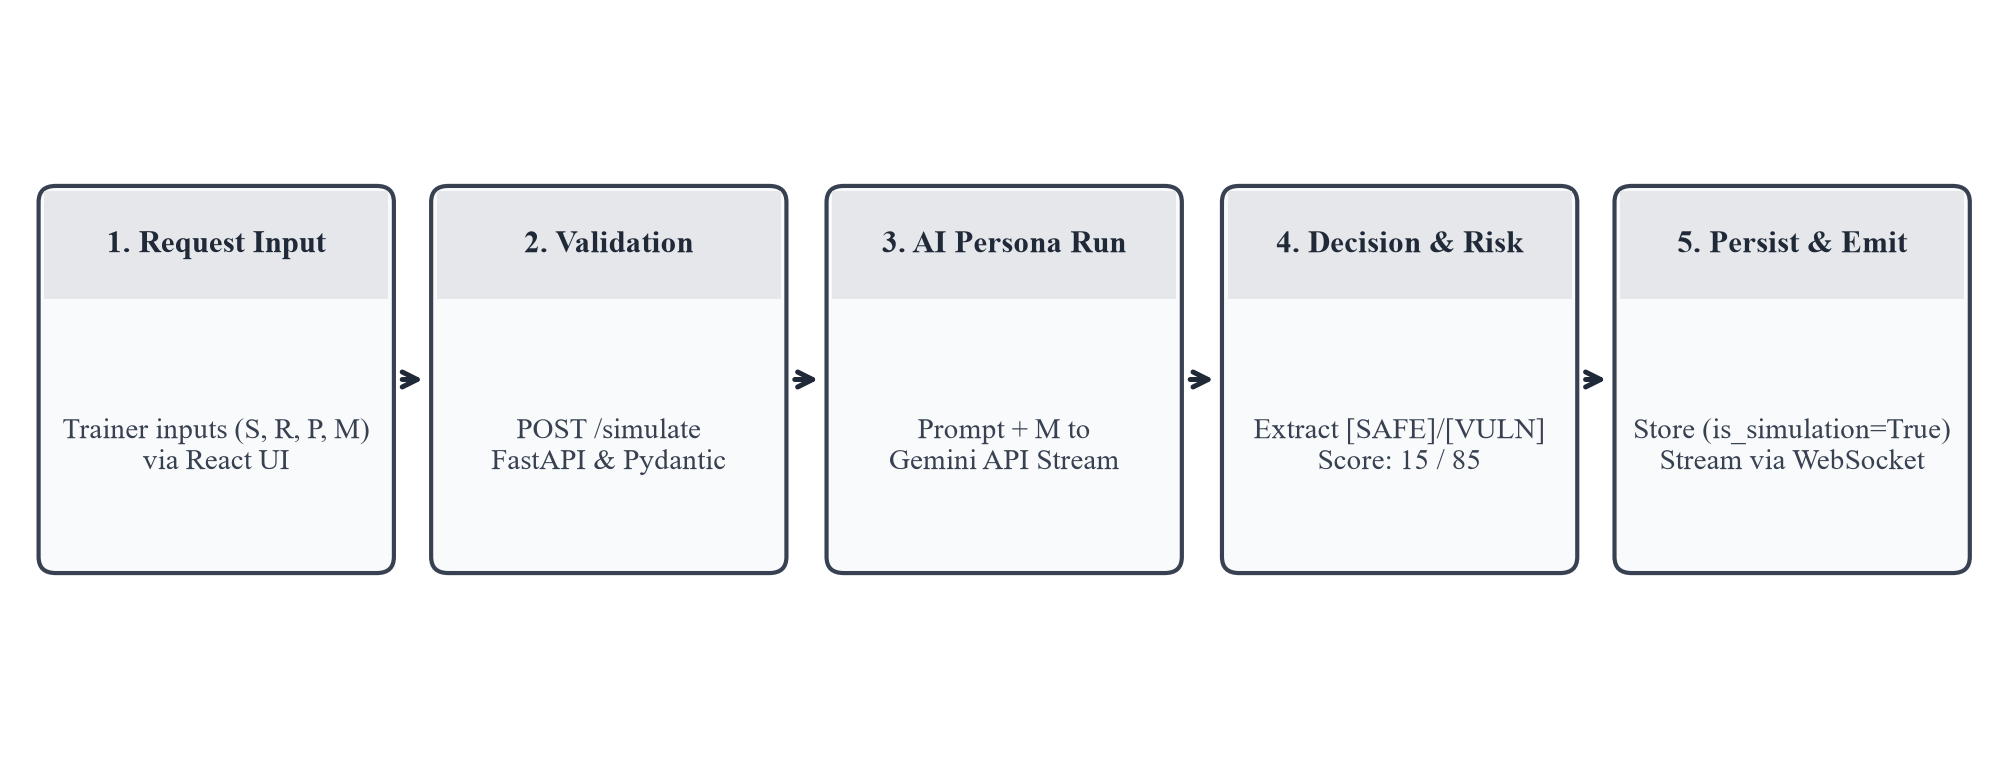
\includegraphics[width=0.82\columnwidth, height=2.5cm, keepaspectratio]{figures/fig2.png}
\caption{Simulation data flow from request validation to stored record.}
\label{fig:data_flow}
\end{figure}

\begin{enumerate}
    \item \textit{Request Ingestion:} The trainer submits the attack scenario $S$, employee role $R$, behavioral profile $P$, and email message $M$ through the React interface.
    \item \textit{Schema Validation:} The FastAPI route handler validates the payload using Pydantic models. If any required field is missing or malformed, an HTTP 400 error is returned immediately.
    \item \textit{Persona Assembly and AI Inference:} The simulation engine retrieves the prompt template corresponding to profile $P$ and role $R$, appends message $M$, and dispatches a single streaming inference request to the Gemini API \cite{gemini2024}.
    \item \textit{Decision Parsing and Risk Scoring:} As tokens stream back, they are forwarded via WebSockets to the client. Upon stream completion, the decision extractor scans for \texttt{[VULNERABLE]} or \texttt{[SAFE]} markers (with keyword fallback). A threat score of $85$ is assigned for vulnerable decisions and $15$ for safe decisions. The score is evaluated by the risk engine to determine severity (Safe, Suspicious, Dangerous).
    \item \textit{Persistence and Telemetry Emission:} An incident record marked with \texttt{is\_simulation = true} and an activity audit entry are committed to the SQLite database via SQLAlchemy. The final assessment payload is emitted to the frontend.
\end{enumerate}

\subsection{System Modules}
The operational logic is encapsulated within five tightly decoupled software modules:
\begin{itemize}
    \item \textbf{Input Ingestion and Validation Module:} Enforces strict data contracts using Pydantic schemas, validating scenario categories, role designations, profile keys, and non-empty subject and body text strings.
    \item \textbf{Agentic Simulation Module:} Manages communication with the Gemini API \cite{gemini2024}. It constructs contextual system prompts that instruct the model to adopt the persona's role, habits, and cognitive constraints, enforcing that all reasoning culminates in a standardized decision marker.
    \item \textbf{Decision Extraction and Parsing Module:} Processes the raw response text from the model, isolating the terminal decision marker. If the explicit marker is obscured, a robust keyword fallback parser analyzes the terminal sentence structure to determine the final classification.
    \item \textbf{Risk Engine Module:} Maps the binary decision to a baseline threat score ($85$ or $15$) and applies enterprise risk thresholds ($\ge 65$ for Dangerous, $35$ to $<65$ for Suspicious, $<35$ for Safe).
    \item \textbf{Persistence and Auditing Module:} Executes atomic database writes via SQLAlchemy \cite{sqlalchemy2024}, storing simulation parameters, reasoning chains, threat scores, confidence values, and execution durations while enforcing logical data segregation.
\end{itemize}

\subsection{Use Case}
The operational use cases available to the Security Trainer role are modeled in Fig. 3. Within the SemanticShield AI system boundary, the trainer can select predefined attack scenarios, configure employee roles and behavioral personas, input phishing text payloads, trigger simulation runs, inspect streaming reasoning outputs, view quantitative risk scores, and review historical threat analytics.

\begin{figure}[t]
\centering
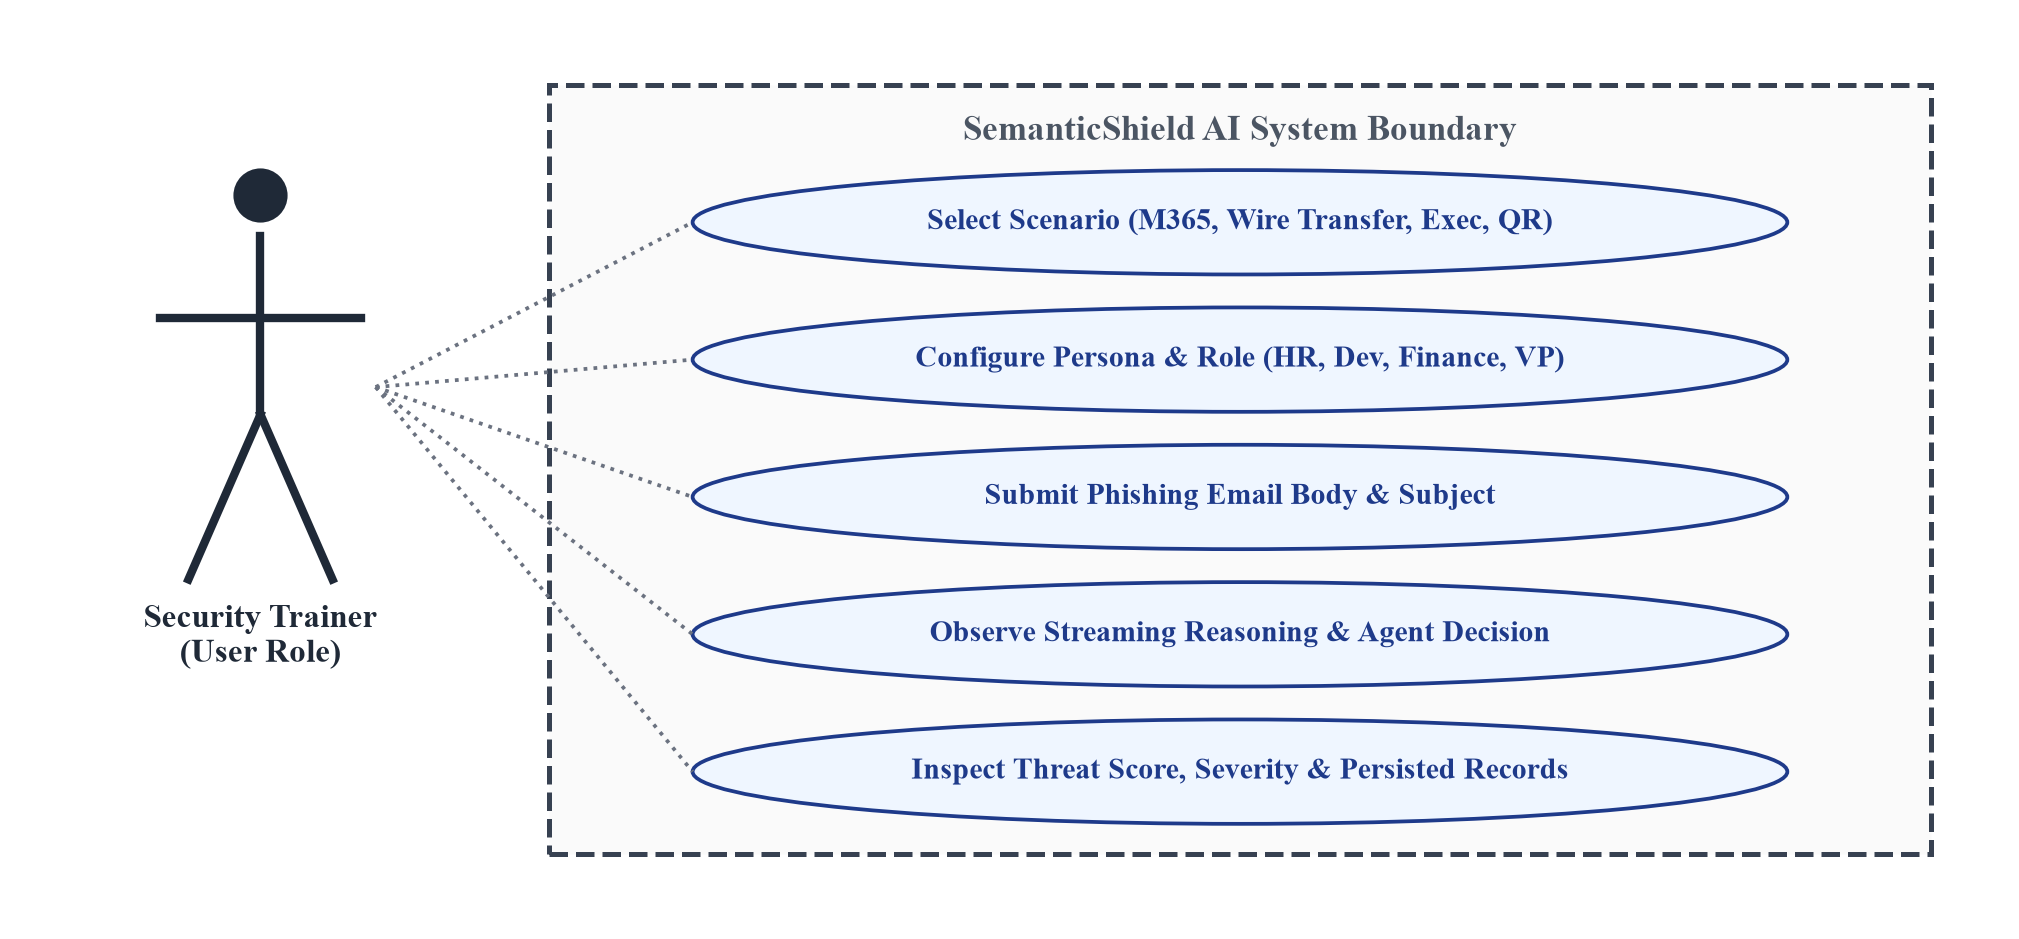
\includegraphics[width=0.80\columnwidth, height=2.6cm, keepaspectratio]{figures/fig3.png}
\caption{Use-case diagram for the trainer role.}
\label{fig:use_case}
\end{figure}

\subsection{Algorithm}
The end-to-end execution flow of the simulation lifecycle is formally defined in Algorithm 1. The procedure accepts the simulation parameters, performs strict input validation, invokes the generative model, extracts the decision marker, maps the threat score, evaluates organizational risk, persists the event, and returns the complete analytical assessment.

\begin{algorithm}[t]
\caption{Processing a simulation request}
\label{alg:simulation}
\begin{algorithmic}[1]
\Require Scenario $S$, role $R$, profile $P$, email subject and body $M$
\Ensure Decision $D$, threat score $T$, stored record
\State Validate $S$, $R$, $P$, and $M$; return error 400 if any value is invalid
\State $prompt \gets \mathrm{SelectPersona}(P)$
\State $response \gets \mathrm{StreamLLM}(prompt, M)$
\State $D \gets \mathrm{ExtractDecision}(response)$, with keyword fallback
\State $T \gets 85\ \mathbf{if}\ D = \mathrm{VULNERABLE},\ \mathbf{otherwise}\ 15$
\State $assessment \gets \mathrm{RiskEngine}(T, categories)$
\State Store incident ($is\_simulation = true$) and activity record
\State \Return reasoning, decision, threat category, severity, and confidence
\end{algorithmic}
\end{algorithm}

\section{METHODOLOGY AND IMPLEMENTATION}

\subsection{Scenario and Target Input}
SemanticShield AI supports four distinct phishing scenario archetypes designed to test different operational vulnerabilities:
\begin{enumerate}
    \item \textit{Microsoft 365 Credential Harvest:} Deceptive security notifications prompting the recipient to re-authenticate or prevent impending password expiration via spoofed landing pages.
    \item \textit{Wire Transfer Fraud:} Pretexting communications masquerading as senior leadership or critical vendors demanding urgent, out-of-band financial transactions.
    \item \textit{Executive Impersonation:} Spear-phishing messages that mimic corporate executives requesting sensitive internal documents, employee records, or gift card acquisitions.
    \item \textit{QR Code Phishing (Quishing):} Emails embedding malicious QR codes that bypass traditional email text scanners, instructing the recipient to scan the code using a mobile device for two-factor authentication or benefits enrollment.
\end{enumerate}

Fig. 4 illustrates the simulation setup interface and completed-run view in the React frontend, allowing the trainer to select scenarios, choose personas, and view real-time outputs.

\begin{figure}[t]
\centering
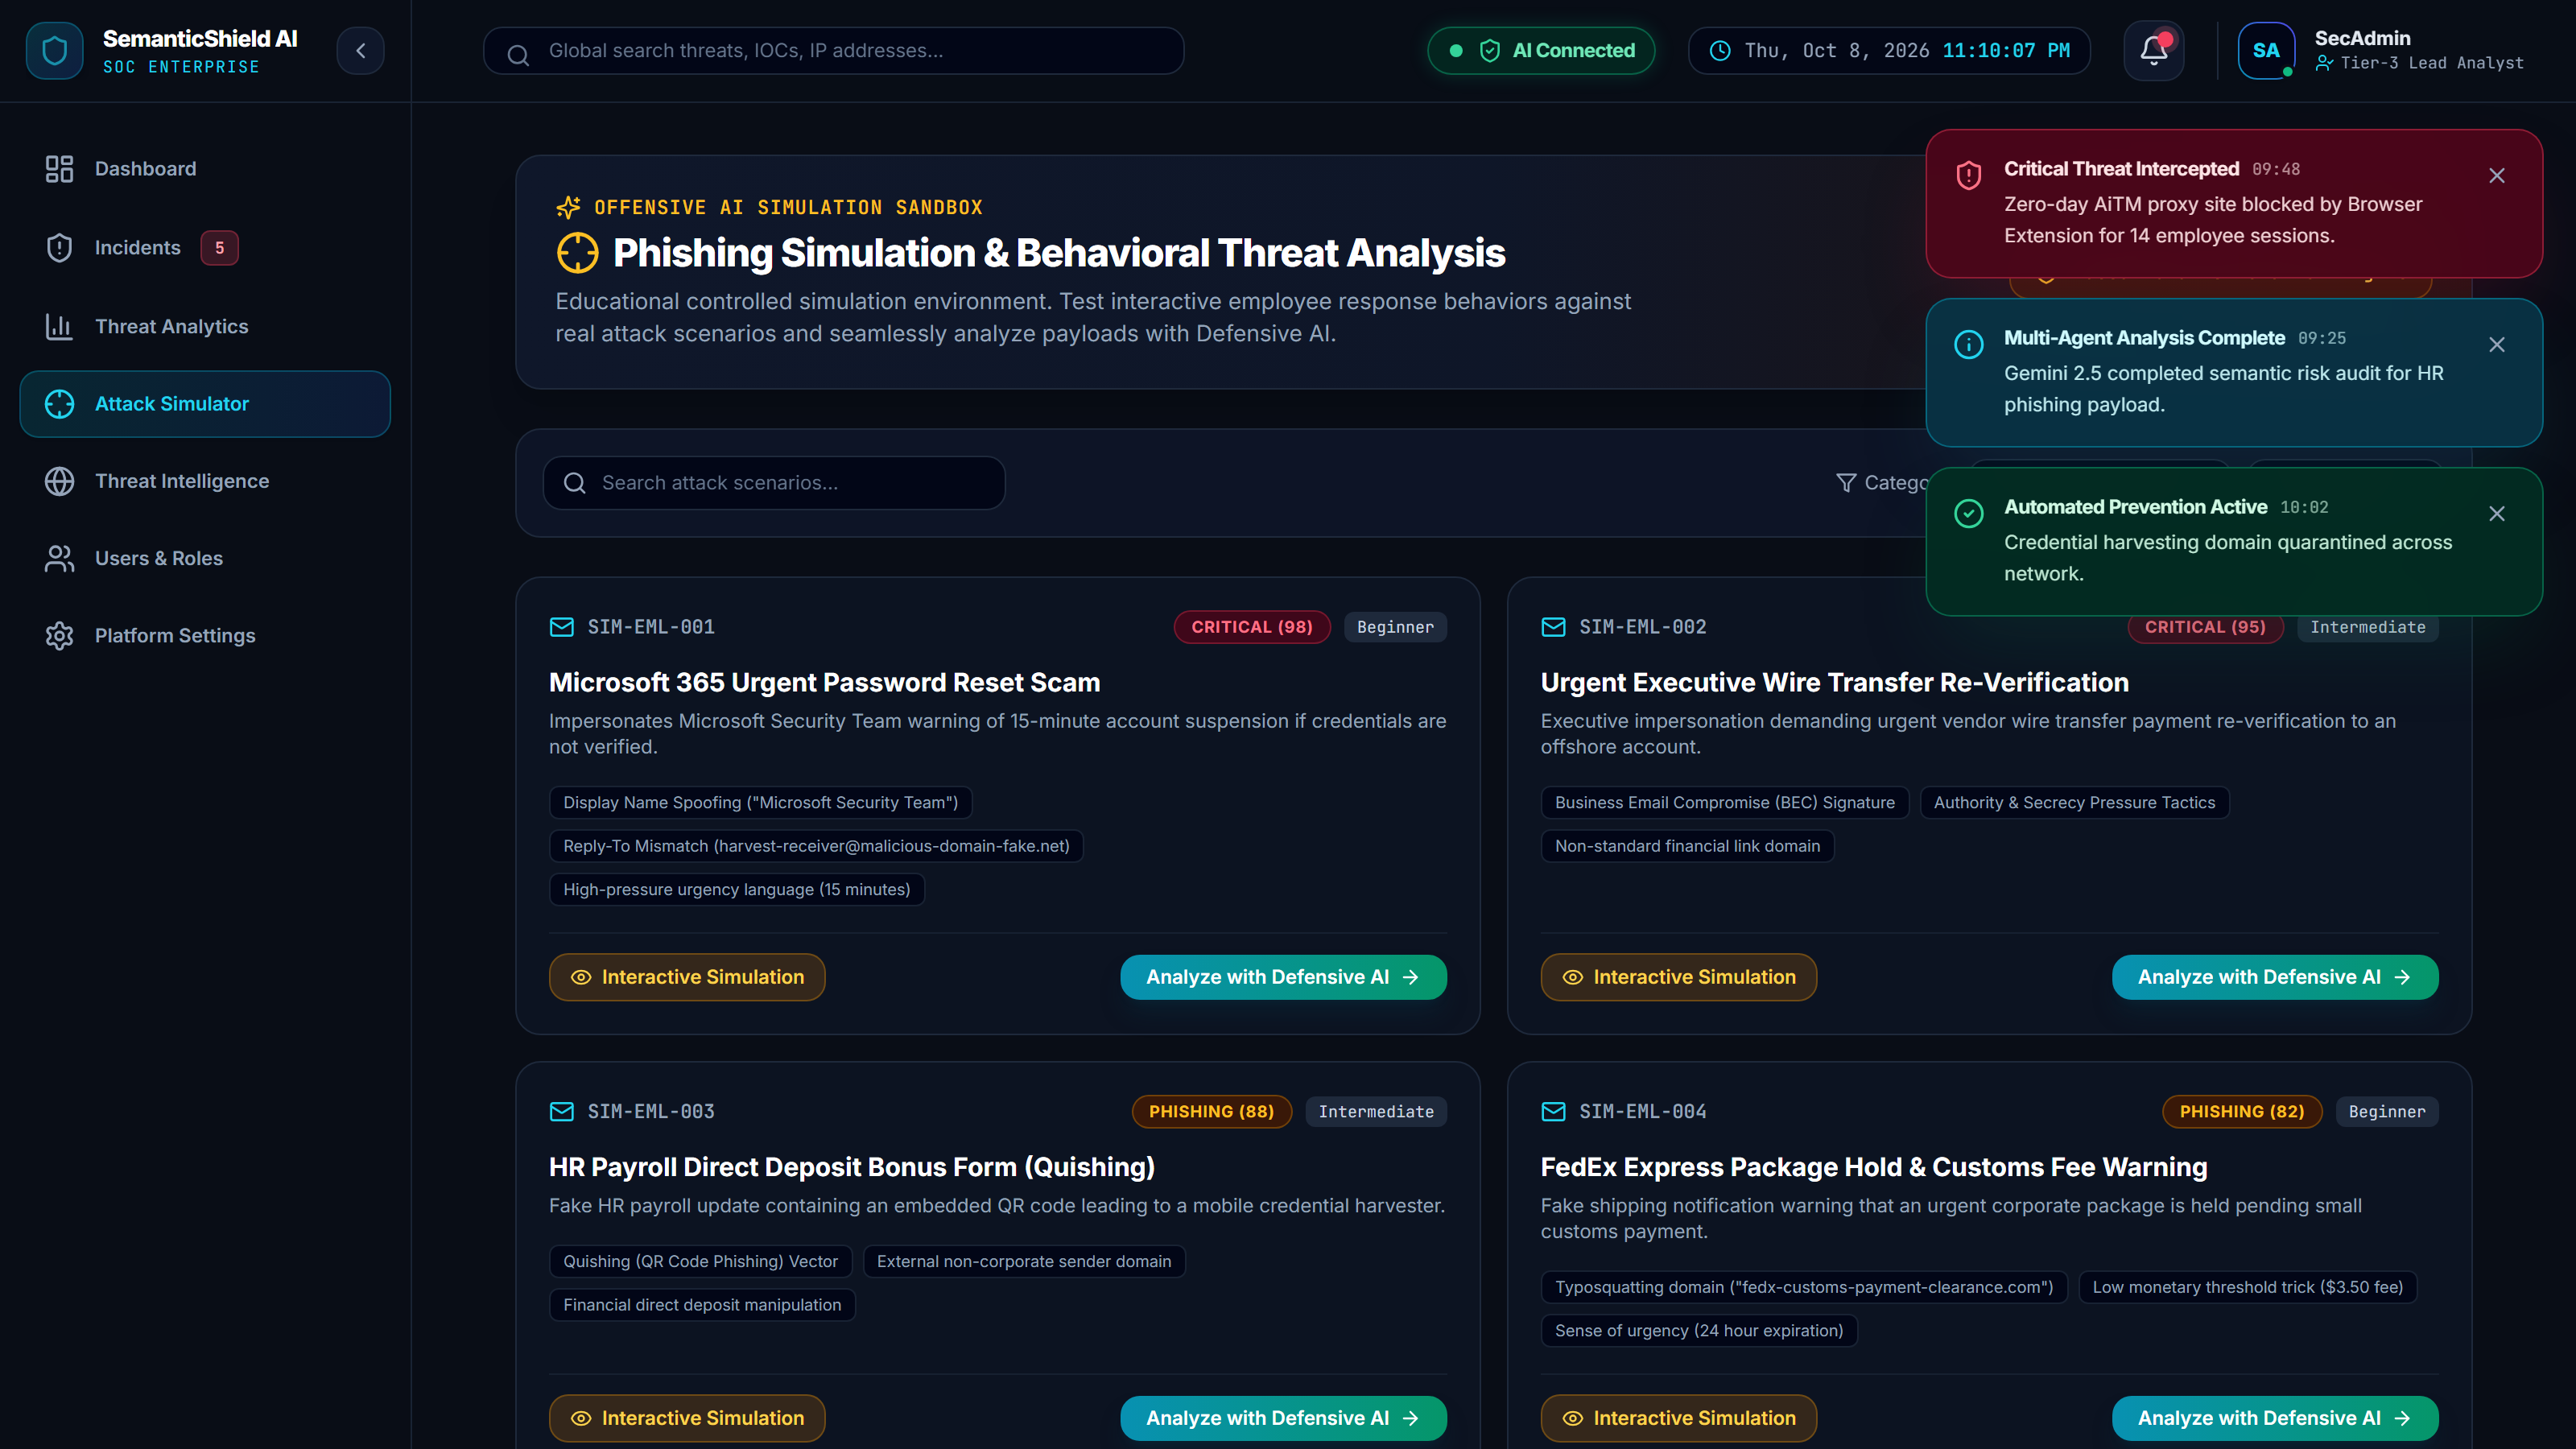
\includegraphics[width=0.82\columnwidth, height=2.6cm, keepaspectratio]{figures/fig4.png}
\caption{Simulation setup and completed-run view. [Placeholder: to be replaced with a real screenshot.]}
\label{fig:simulator_setup}
\end{figure}

\subsection{Behavioral Persona Design}
To capture realistic organizational diversity, SemanticShield AI implements four behavioral personas, detailed in Table \ref{tab:comparison_profiles}. Each persona represents a specific organizational role and embodies distinct cognitive habits, verification routines, and failure modes:
\begin{itemize}
    \item \textbf{Trusting (HR Manager):} Characterized by high interpersonal trust, professional politeness, and a drive to resolve employee inquiries promptly. This persona prioritizes customer service and internal support, routinely accepting urgent requests without inspecting underlying hyperlink destinations.
    \item \textbf{Security-Conscious (Developer):} Emphasizes technical skepticism and methodical verification. This persona scrutinizes email headers, examines sender domains, inspects URLs for typosquatting, and verifies authentication protocols before interacting with message elements.
    \item \textbf{Overwhelmed (Finance Manager):} Operates under continuous cognitive load and severe time constraints. Prioritizing fiscal deadlines and operational throughput, this persona frequently bypasses verification steps when confronted with messages asserting urgent billing issues or service interruptions.
    \item \textbf{Executive (Vice President):} Manages extensive volumes of strategic correspondence, frequently processing messages on mobile devices while traveling. This persona relies on brand authority and executive context, skimming emails quickly and delegating or complying when messages appear relevant to organizational operations.
\end{itemize}

\begin{table*}[t]
\caption{Behavioral Profile Specifications and Cognitive Characteristics}
\label{tab:comparison_profiles}
\centering
\renewcommand{\arraystretch}{0.90}
\begin{tabularx}{\textwidth}{lp{2.5cm}Xp{3.5cm}X}
\toprule
\textbf{Profile} & \textbf{Representative Role} & \textbf{Core Behavioral Habit} & \textbf{Primary Heuristic Checked} & \textbf{Common Failure Mode} \\
\midrule
Trusting & HR Manager & High interpersonal benevolence; quick execution & Courtesy, sender authority, organizational context & Assumes legitimacy of urgent employee/vendor requests without URL checking \\
\addlinespace
Security-Conscious & Software Developer & Analytical inspection; technical skepticism & Technical headers, domain authenticity, exact URL structure & Rare failure under subtle homograph domains or complex OAuth consent grants \\
\addlinespace
Overwhelmed & Finance Manager & High workload; acute deadline urgency & Task actionability and deadline immediacy over security & Clicks through warnings under time pressure to resolve perceived financial blocks \\
\addlinespace
Executive & Vice President & Rapid mobile triage; high-level delegation & Brand authority and organizational relevance & Skims messages rapidly on mobile devices, trusting executive framing \\
\bottomrule
\end{tabularx}
\end{table*}

\subsection{LLM Reasoning and Decision Extraction}
The simulation engine executes exactly one model call per simulation run using the Gemini API \cite{gemini2024}. The prompt structure combines a system instruction defining the behavioral persona with the candidate phishing subject and body. The model is strictly instructed to produce its analysis in two sequential segments:
\begin{enumerate}
    \item \textit{Reasoning Chain:} A natural language explanation detailing how the persona perceives the message, what visual or technical elements it examines, and what cognitive trade-offs determine its reaction.
    \item \textit{Decision Marker:} A standardized closing marker consisting exclusively of \texttt{[VULNERABLE]} or \texttt{[SAFE]}.
\end{enumerate}

To ensure deterministic decision capture, the backend parses the completion stream using a pattern matcher that targets the final bracketed marker. If the model generates an anomalous token sequence lacking the exact delimiter, a keyword fallback routine inspects the terminal sentences for positive assertions of compliance (e.g., ``I will click the link'', ``entering credentials'') or defense (e.g., ``reporting to security'', ``ignoring fraudulent email''), mapping them reliably to \texttt{VULNERABLE} or \texttt{SAFE}.

\subsection{Threat Scoring and Risk Integration}
Once the decision $D$ is extracted, it is transformed into a calibrated threat score $T$:
\begin{equation}
T = \begin{cases} 
85, & \text{if } D = \text{\texttt{VULNERABLE}} \\
15, & \text{if } D = \text{\texttt{SAFE}}
\end{cases}
\end{equation}

The threat score is passed directly to the organizational risk engine. The risk engine enforces standardized categorization thresholds:
\begin{itemize}
    \item \textbf{Dangerous:} $T \ge 65$ (Score $85$, indicating successful compromise).
    \item \textbf{Suspicious:} $35 \le T < 65$ (Intermediate risk boundary).
    \item \textbf{Safe:} $T < 35$ (Score $15$, indicating successful detection).
\end{itemize}

In addition, the risk engine calculates an analytical confidence score ranging between $90\%$ and $98\%$, reflecting the semantic certainty of the model's decision markers and reasoning consistency.

\subsection{Incident Logging and Persistence}
All simulation events are persisted to the SQLite database via SQLAlchemy \cite{sqlalchemy2024}. A foundational design requirement is that simulated attacks must never corrupt or pollute real enterprise security operations. Therefore, every simulation run creates an incident record with the explicit database flag:
\begin{equation}
\texttt{is\_simulation} = \texttt{true}
\end{equation}

This guarantees that security analysts can filter out synthetic evaluations during real incident triage while retaining historical telemetry for behavioral analytics. Concurrently, an activity record is written to the audit feed table, logging the trainer ID, timestamp, profile, scenario, threat score, and response latency.

Fig. 5 shows the main analytics dashboard in light theme, visualizing aggregated simulation results, threat severity trends, and activity logs.

\begin{figure}[t]
\centering
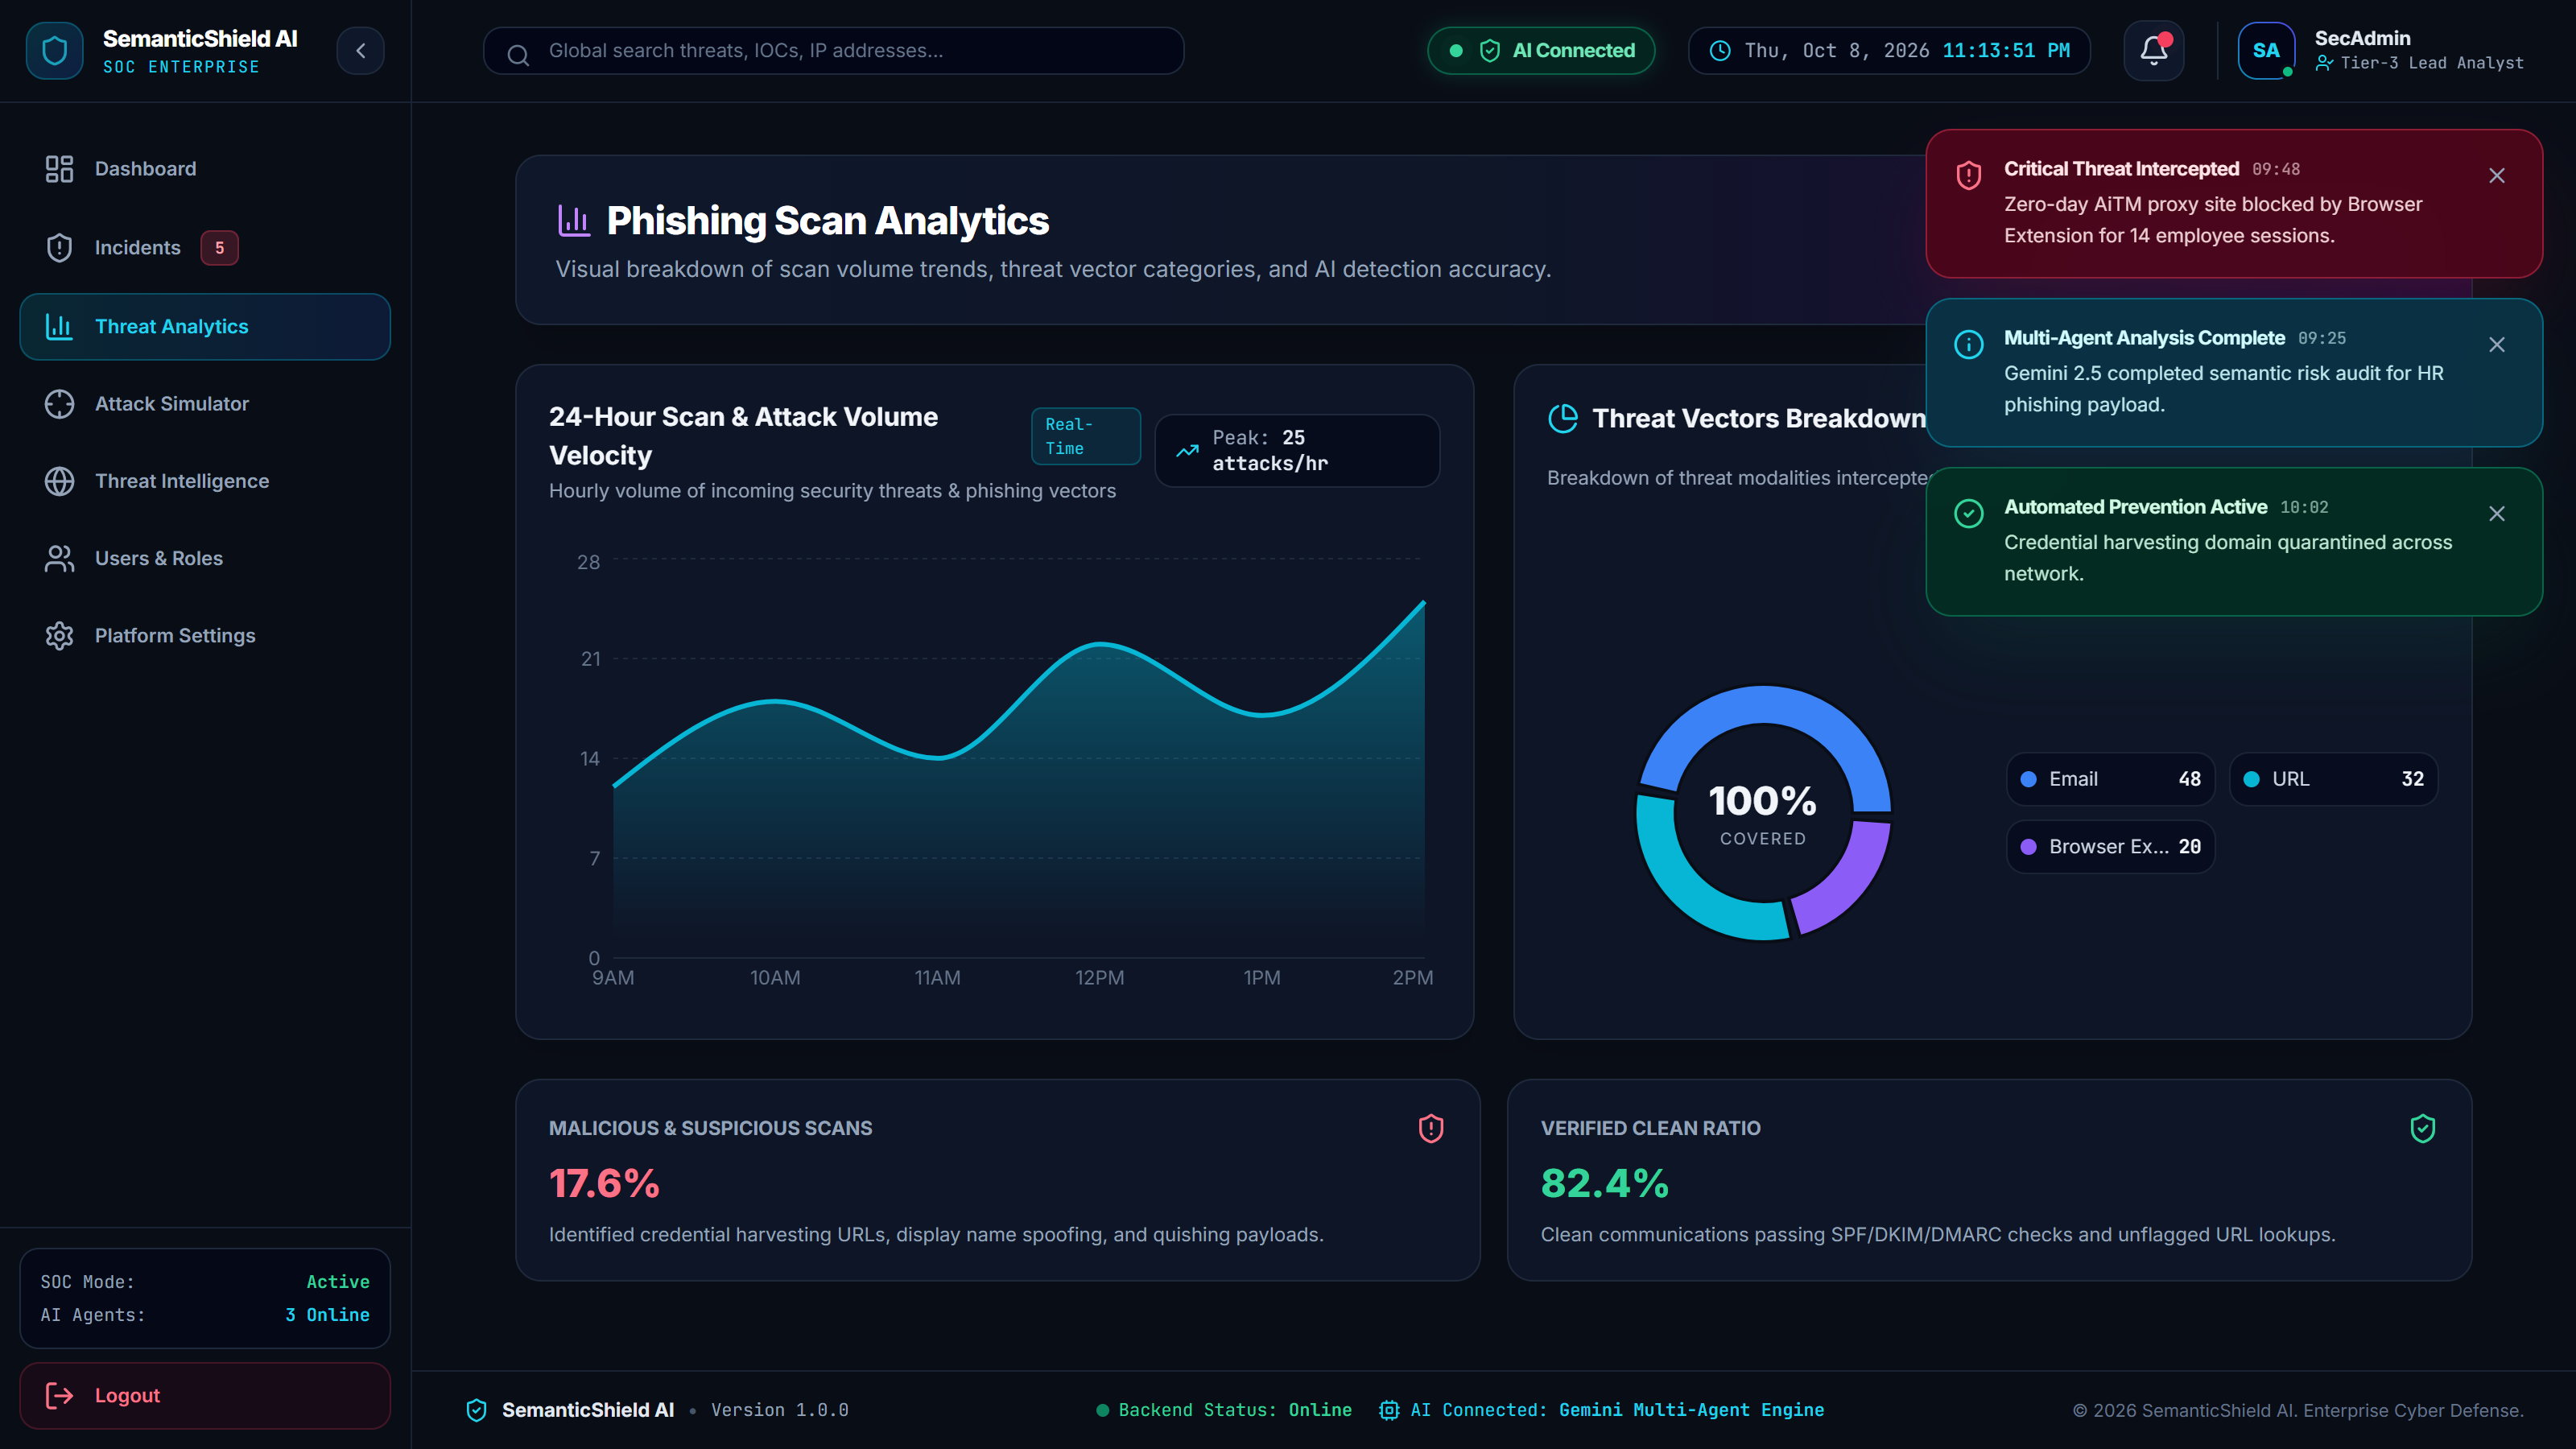
\includegraphics[width=0.82\columnwidth, height=2.6cm, keepaspectratio]{figures/fig5.png}
\caption{Main analytics dashboard in light theme. [Placeholder: to be replaced with a real screenshot.]}
\label{fig:analytics_dashboard}
\end{figure}

\subsection{Technology Stack}
The complete technology stack of SemanticShield AI is summarized in Table \ref{tab:tech_stack}. In strict adherence to architectural modularity, the system uses only Python, FastAPI, SQLite, SQLAlchemy, Alembic, React, WebSocket, and the Gemini API.

\begin{table}[t]
\caption{System Technology Stack by Architectural Layer}
\label{tab:tech_stack}
\centering
\renewcommand{\arraystretch}{0.90}
\begin{tabularx}{\columnwidth}{llX}
\toprule
\textbf{Layer} & \textbf{Technology} & \textbf{Architectural Function} \\
\midrule
Frontend & React & Single-page interface, real-time telemetry rendering \\
Real-Time & WebSocket & Full-duplex persistent stream for reasoning telemetry \\
Backend & FastAPI & Asynchronous REST routing and Pydantic validation \\
Runtime & Python & Python 3.10+ execution environment \\
AI Model & Gemini API & Persona emulation and chain-of-thought inference \\
Database & SQLite & Embedded ACID-compliant relational data storage \\
ORM & SQLAlchemy & Declarative database models and relationship queries \\
Migrations & Alembic & Schema version control and database revisions \\
\bottomrule
\end{tabularx}
\end{table}

\subsection{Software and Hardware Requirements}
The operational requirements for deploying SemanticShield AI are outlined in Table \ref{tab:requirements}. All specified hardware values represent recommended guidelines rather than measured empirical thresholds.

\begin{table}[t]
\caption{Software and Hardware Requirements (Recommended)}
\label{tab:requirements}
\centering
\renewcommand{\arraystretch}{0.90}
\begin{tabularx}{\columnwidth}{lp{2.6cm}X}
\toprule
\textbf{Category} & \textbf{Component} & \textbf{Recommended Specification} \\
\midrule
Runtime & Python Environment & Python 3.10 or later \\
Core Libraries & Web \& Persistence & FastAPI, Pydantic, SQLAlchemy, Alembic \\
Client Framework & Frontend & React single-page application \\
Communication & Transport Protocol & WebSocket real-time transport \\
AI Integration & Cloud API & Outbound HTTPS to Gemini API \\
Processor (CPU) & Recommended Compute & 4-core 2.5 GHz or higher (recommended) \\
Memory (RAM) & Recommended Memory & 8 GB RAM (recommended) \\
Storage & Recommended Disk & 10 GB SSD available storage (recommended) \\
Network & Recommended Bandwidth & Stable broadband Internet connection \\
\bottomrule
\end{tabularx}
\end{table}

\section{RESULTS AND DISCUSSION}

\subsection{Evaluation Setup}
To evaluate the behavioral simulation capabilities of SemanticShield AI, an empirical experiment comprising 63 distinct simulation runs was conducted. All 63 runs evaluated the exact same phishing payload to maintain rigorous experimental control across behavioral personas.

The attack payload simulated a Microsoft 365 credential-harvesting attempt. The email subject was configured as ``URGENT: Microsoft 365 Password Expiration Notification'', and the body warned the recipient that their enterprise cloud account password would expire within 24 hours, instructing them to retain their current credentials by clicking an embedded verification hyperlink. The embedded hyperlink directed the user to a deceptive domain: \texttt{microsoft-security.com} instead of the legitimate corporate domain \texttt{microsoft.com}.

The 63 evaluation runs were distributed across the four behavioral profiles:
\begin{itemize}
    \item \textbf{Trusting (HR Manager):} 18 runs.
    \item \textbf{Security-Conscious (Developer):} 16 runs.
    \item \textbf{Overwhelmed (Finance Manager):} 15 runs.
    \item \textbf{Executive (VP):} 14 runs.
\end{itemize}

\textit{Qualitative Demonstration Example:} In a direct qualitative comparison on this identical email, the Trusting profile (HR Manager) exhibited immediate vulnerability. The agent's reasoning noted the official Microsoft branding, conveyed concern over potential administrative disruption to employee communications, and concluded that complying promptly was the most responsible action, outputting \texttt{[VULNERABLE]}. In contrast, the Security-Conscious profile (Developer) methodically inspected the hyperlink, recognized that \texttt{microsoft-security.com} was an external, unauthorized domain attempting typosquatting, concluded that Microsoft does not solicit password retentions via third-party domains, and output \texttt{[SAFE]}. This qualitative contrast illustrates how the persona prompts successfully induce realistic cognitive divergence.

\subsection{Decision Outcomes by Profile}
The distribution of simulation decisions across all 63 evaluation runs is illustrated in Fig. 6.

\begin{figure}[t]
\centering
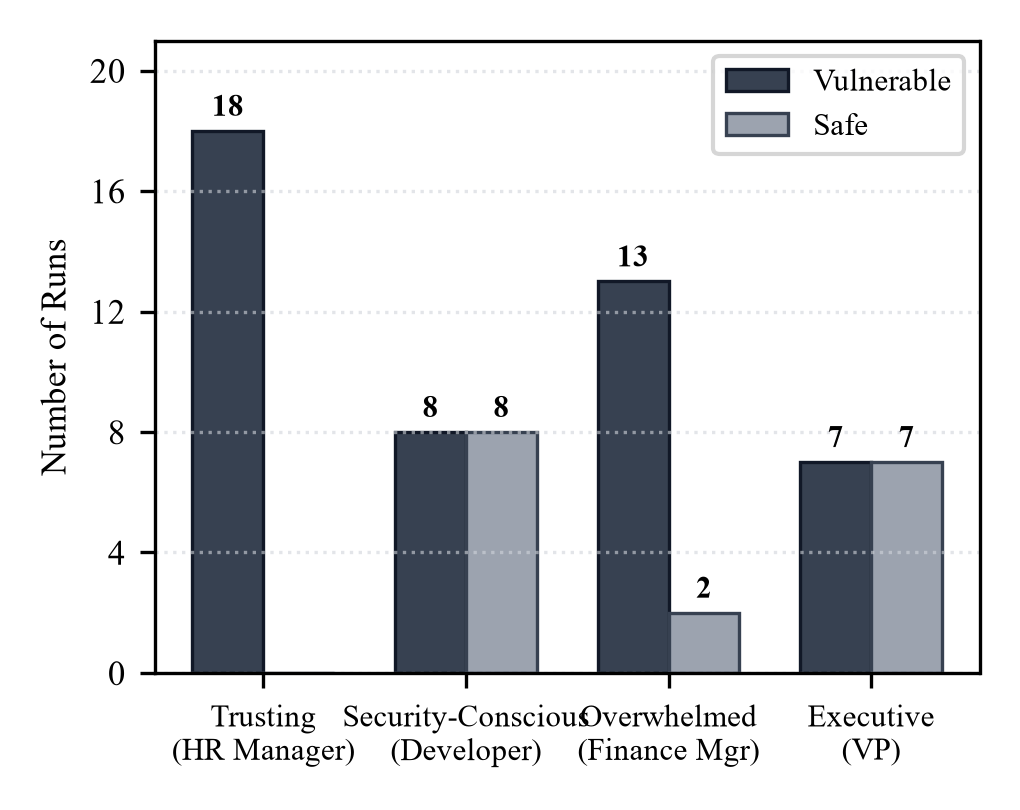
\includegraphics[width=0.72\columnwidth, height=2.3cm, keepaspectratio]{figures/fig6.png}
\caption{Agent decisions by behavior profile (Safe vs Vulnerable) across 63 runs.}
\label{fig:decisions}
\end{figure}

The empirical results reveal pronounced differences in vulnerability across personas:
\begin{itemize}
    \item \textbf{Trusting (HR Manager):} Recorded 0 Safe decisions and 18 Vulnerable decisions across 18 runs, exhibiting a 100\% vulnerability rate. The persona consistently prioritized administrative compliance and service continuity over domain scrutiny.
    \item \textbf{Security-Conscious (Developer):} Recorded 8 Safe decisions and 8 Vulnerable decisions across 16 runs, achieving a 50\% defensive success rate. While the persona frequently caught the spoofed domain, nuanced variations in the reasoning chain occasionally prioritized avoiding system lockouts.
    \item \textbf{Overwhelmed (Finance Manager):} Recorded 2 Safe decisions and 13 Vulnerable decisions across 15 runs, demonstrating an 86.7\% vulnerability rate. Under simulated workload stress and urgency, the persona repeatedly bypassed verification.
    \item \textbf{Executive (VP):} Recorded 7 Safe decisions and 7 Vulnerable decisions across 14 runs, resulting in a 50\% vulnerability rate. The executive persona's focus on operational relevance occasionally led to quick approval, while high-level skepticism preserved safety in half the trials.
\end{itemize}

Across all 63 runs, the system produced 46 Vulnerable outcomes and 17 Safe outcomes.

\subsection{Severity and Confidence}
The distribution of threat severity classifications produced by the risk engine across all 63 simulation runs is depicted in Fig. 7.

\begin{figure}[t]
\centering
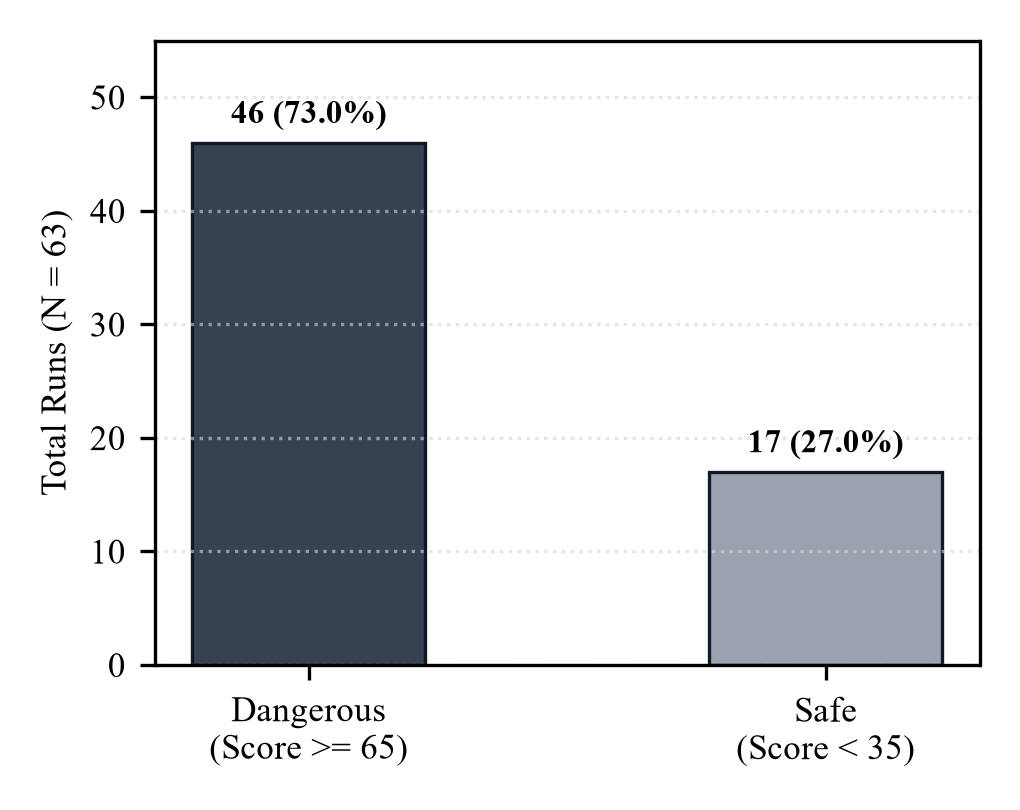
\includegraphics[width=0.72\columnwidth, height=2.3cm, keepaspectratio]{figures/fig7.png}
\caption{Distribution of threat severity levels across all runs.}
\label{fig:severity}
\end{figure}

Following the risk engine threshold rules, the 46 Vulnerable outcomes mapped to threat scores of $85$, receiving the severity label \textbf{Dangerous}. The 17 Safe outcomes mapped to threat scores of $15$, receiving the severity label \textbf{Safe}. No simulation outcomes fell into the intermediate Suspicious category, as the binary decision mapping produced distinct scores ($85$ and $15$).

\begin{figure}[t]
\centering
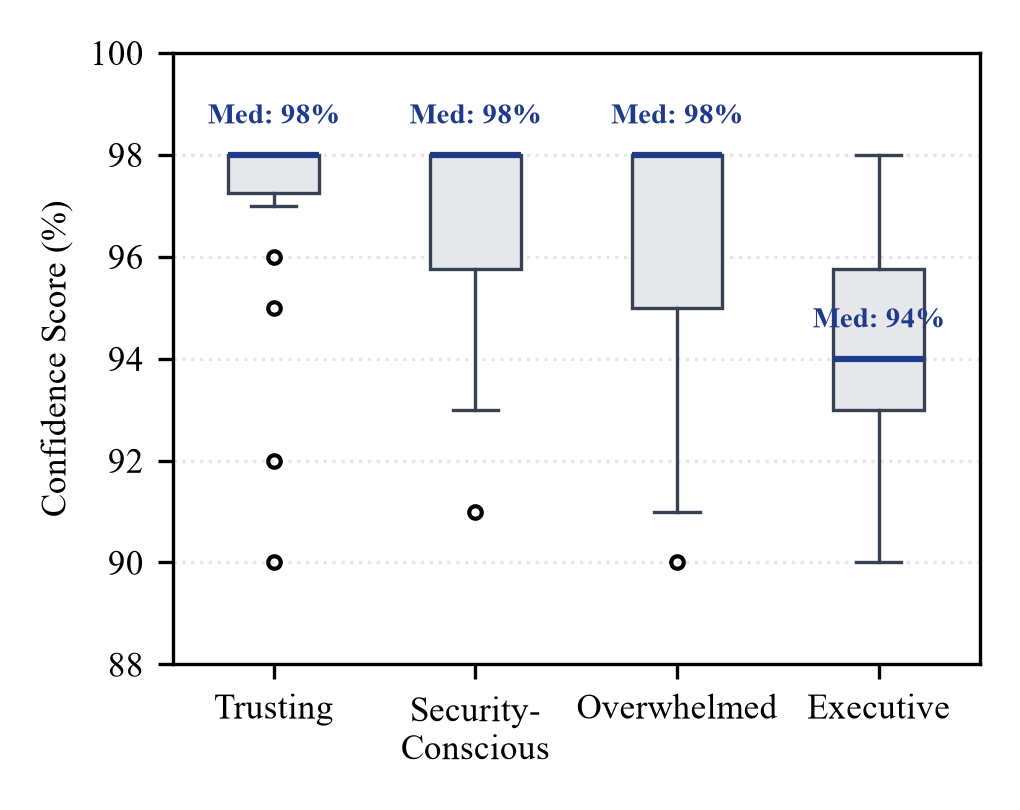
\includegraphics[width=0.72\columnwidth, height=2.3cm, keepaspectratio]{figures/fig8.png}
\caption{Confidence score distribution by behavior profile.}
\label{fig:confidence}
\end{figure}

Fig. 8 illustrates the distribution of analytical confidence scores across behavioral profiles. Across all 63 evaluations, all confidence scores fell within the narrow range of $90\%$ to $98\%$. The median confidence score was exactly $98\%$ for the Trusting, Security-Conscious, and Overwhelmed profiles, and $94\%$ for the Executive profile. This high confidence reflects the semantic decisiveness of the model's reasoning chains and the unambiguous nature of the extracted decision markers.

\subsection{Response Duration}
The execution duration of each simulation run was tracked from request dispatch to terminal database persistence. Fig. 9 illustrates the mean response duration across the four behavioral profiles.

\begin{figure}[t]
\centering
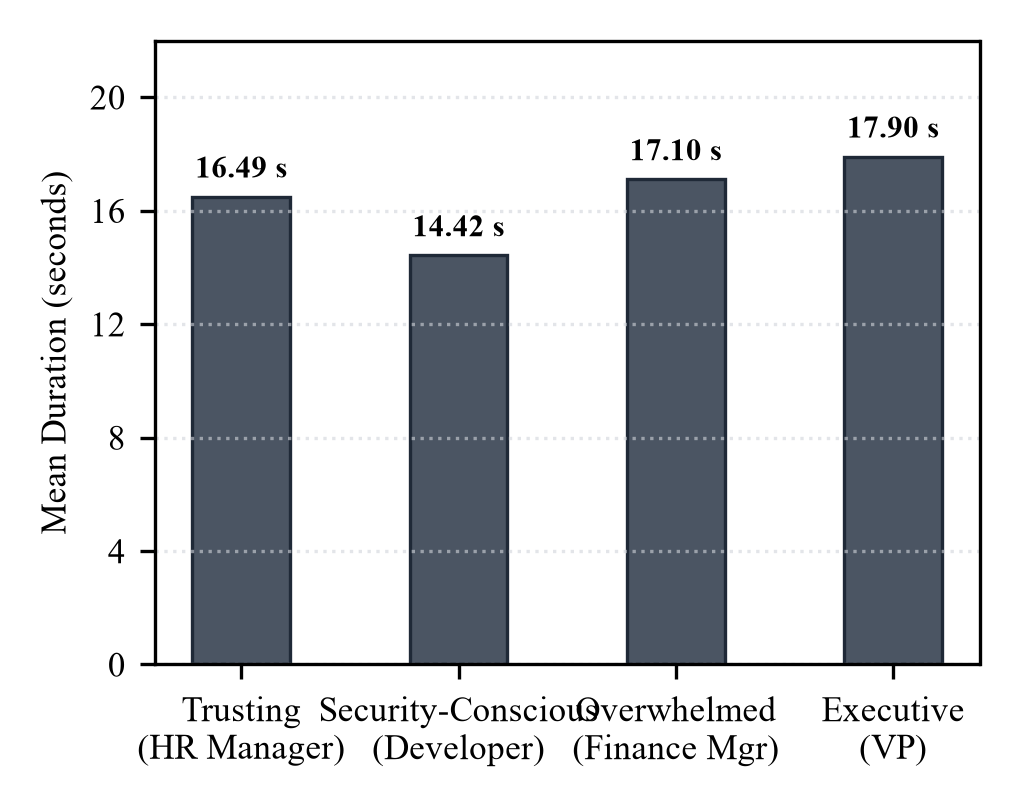
\includegraphics[width=0.72\columnwidth, height=2.3cm, keepaspectratio]{figures/fig9.png}
\caption{Average simulation duration by behavior profile.}
\label{fig:duration}
\end{figure}

The mean durations recorded per profile were: Trusting (HR Manager) 16.49~s, Security-Conscious (Developer) 14.42~s, Overwhelmed (Finance Manager) 17.10~s, and Executive (VP) 17.90~s. The variations in latency correlate directly with reasoning chain complexity. The Security-Conscious persona generated concise, technical inspections of the domain, yielding the shortest average duration (14.42~s). Conversely, the Executive persona generated longer, more elaborate chain-of-thought reflections balancing corporate risk, travel constraints, and delegation protocols, resulting in the highest average latency (17.90~s).

\subsection{Discussion and Limitations}
The empirical results demonstrate that SemanticShield AI successfully models cognitive divergence across simulated enterprise personas without exposing human employees to deceptive phishing emails. The high vulnerability rates observed in the Trusting and Overwhelmed personas align with established social engineering literature \cite{hadnagy2018}, validating that simulated time pressure and customer-centric habits significantly degrade verification discipline.

\textit{Research Limitations:} Several important limitations must be noted:
\begin{enumerate}
    \item \textit{Sample Size and Scenario Scope:} 63 runs were conducted against a single credential-harvesting scenario. Evaluating other scenarios may yield different susceptibility patterns.
    \item \textit{Absence of Human Participant Studies:} The study did not include a human participant baseline; results describe model behavior under these personas, not the behavior of real employees.
    \item \textit{Synthetic Persona Modeling:} While persona prompts simulate workplace habits, they cannot fully reproduce all unpredictable environmental factors influencing real human decisions.
\end{enumerate}

\section{CONCLUSION AND FUTURE SCOPE}

\subsection{Conclusion}
This paper presented SemanticShield AI, an intelligent agent framework for phishing simulation and behavioral threat analysis. By combining the Gemini API with structured persona prompts, the system emulates the cognitive responses and failure modes of diverse employee roles without sending deceptive emails to real employees. Across 63 empirical simulation runs on a credential-harvesting payload, the system demonstrated distinct behavioral divergence, recording a 100\% vulnerability rate in Trusting HR personas, 86.7\% in Overwhelmed Finance personas, and 50\% in both Security-Conscious Developers and Executive personas. Transparent reasoning chains, automated decision extraction, calibrated threat scoring ($85$ for Dangerous, $15$ for Safe), and strict database isolation (\texttt{is\_simulation = true}) provide security teams with actionable, ethical insights into human-factor vulnerabilities.

\subsection{Future Scope}
Future research directions will expand upon these foundations:
\begin{itemize}
    \item \textbf{Multi-Turn Phishing:} Expanding the simulation engine to support dynamic, multi-turn conversational social engineering over chat and email threads.
    \item \textbf{Multi-Modal Attack Vectors:} Incorporating evaluation of multi-modal phishing attacks, including voice phishing (vishing) and malicious document attachments.
    \item \textbf{Dynamic Scenario Generation:} Implementing automated generative threat actors that dynamically adapt phishing scenarios based on a profile's historical defensive weaknesses.
    \item \textbf{Enterprise Identity Integration:} Integrating with enterprise directory services to automatically generate customized persona profiles reflecting real departmental organizational structures.
    \item \textbf{Human-in-the-Loop Validation:} Conducting controlled user studies to correlate synthetic persona vulnerability predictions with actual anonymized human testing data.
\end{itemize}

\begin{thebibliography}{99}
\bibitem{russell2021} S. Russell and P. Norvig, \textit{Artificial Intelligence: A Modern Approach}, 4th ed. Pearson, 2021.
\bibitem{wooldridge1995} M. Wooldridge and N. R. Jennings, ``Intelligent agents: Theory and practice,'' \textit{The Knowledge Engineering Review}, vol. 10, no. 2, pp. 115--152, 1995.
\bibitem{brown2020} T. Brown \textit{et al.}, ``Language models are few-shot learners,'' in \textit{Advances in Neural Information Processing Systems}, vol. 33, pp. 1877--1901, 2020.
\bibitem{lewis2020} P. Lewis \textit{et al.}, ``Retrieval-augmented generation for knowledge-intensive NLP tasks,'' in \textit{Advances in Neural Information Processing Systems}, vol. 33, pp. 9459--9474, 2020.
\bibitem{zhao2023} W. X. Zhao \textit{et al.}, ``A survey of large language models,'' arXiv:2303.18223, 2023.
\bibitem{dhamija2006} R. Dhamija, J. D. Tygar, and M. Hearst, ``Why phishing works,'' in \textit{Proc. SIGCHI Conf. Human Factors in Computing Systems (CHI)}, 2006.
\bibitem{kumaraguru2010} P. Kumaraguru \textit{et al.}, ``Teaching Johnny not to fall for phish,'' \textit{ACM Transactions on Internet Technology}, vol. 10, no. 2, 2010.
\bibitem{sheng2007} S. Sheng \textit{et al.}, ``Anti-phishing Phil: The design and evaluation of a game that teaches people not to fall for phish,'' in \textit{Proc. Symposium on Usable Privacy and Security (SOUPS)}, 2007.
\bibitem{hadnagy2018} C. Hadnagy, \textit{Social Engineering: The Science of Human Hacking}, 2nd ed. Wiley, 2018.
\bibitem{verizon2024} Verizon, ``2024 Data Breach Investigations Report,'' Verizon Business, 2024.
\bibitem{gemini2024} Google, ``Gemini API documentation,'' Google AI for Developers. [Online]. Available: https://ai.google.dev/gemini-api/docs
\bibitem{fastapi2024} S. Ram\'irez, ``FastAPI documentation.'' [Online]. Available: https://fastapi.tiangolo.com
\bibitem{sqlalchemy2024} SQLAlchemy and Alembic projects, ``SQLAlchemy documentation'' and ``Alembic documentation.'' [Online]. Available: https://docs.sqlalchemy.org and https://alembic.sqlalchemy.org
\end{thebibliography}

\end{document}
